\chapter[O Estudo de Caso]{O Estudo de Caso}

Neste capítulo será apresentado o estudo de caso desse trabalho. Na primeira seção será apresentado o contexto e a caracterização da organização do estudo de caso. Na segunda seção será apresentada a empresa contratada para o desenvolvimento do projeto. Na terceira seção será apresentada a caracterização do contrato e o objeto do contrato, ou seja, a caracterização do projeto que os dados foram coletados. Na quarta seção será apresentada a solução aplicada na gestão do contrato analisado. E, finalmente, na quinta seção serão apresentadas a análise dos dados e a discussão dos resultados.

\section[A Organização]{A Organização}

O órgão escolhido, IPHAN, possui uma força de trabalho atuante na área de TI de apenas 8 funcionários, dos quais apenas 3 trabalham diretamente com sistemas. O perfil dessa equipe é apresentado na Tab. (3). Devido ao número reduzido de servidores disponíveis na área de TI do órgão, frequentemente uma mesma pessoa acaba desempenhando diferentes papeis requeridos pela Instrução Normativa MP/SLTI Nº04/2010.

\begin{table}[H]
\center
\footnotesize
\begin{tabular}{|c|c|c|}
\hline
\textbf{Área}          & \textbf{Perfil}   & \textbf{Quantidade} \\ \hline
TI Geral               & Coordenador de Tecnologia da Informação   & 1                   \\ \hline
Infraestrutura         & Analista de Tecnologia da Informação   & 2                   \\ \hline
Sistemas               & Analista de Tecnologia da Informação   & 2                   \\ \hline
\multirow{3}{*}{Apoio} & Analista de Tecnologia da Informação    & 1                   \\ \cline{2-3} 
\multicolumn{1}{|l|}{} & Servidor do Ministério da Ciência, Tecnologia e Inovação & 1                   \\ \cline{2-3} 
\multicolumn{1}{|l|}{} & Servidor do IPHAN & 1                   \\ \hline
\end{tabular}
\caption{Perfil da Equipe}
\end{table}

O contexto atual do órgão foi identificado por meio da aplicação da técnica de entrevista informal, de questionário e da documentação disponível do órgão. O questionário aplicado pode ser encontrado no Apêndice I - Questionário Gestão do Contrado. Vale ressaltar que esse questionário foi aplicado não só para caracterização da organização como também para coleta de dados necessários para o estudo de caso desse trabalho e ele foi projetado de forma generalizada para que tanto o IPHAN quanto a empresa contratada, EGL - Engenharia, pudessem respondê-lo.
 
Os fatores mais significantes que são gerenciados pela área de TI do órgão são:
\begin{itemize}
\item Atender as demandas para desenvolvimento de sistemas (sistema novo, manutenção, documentação).
\item Controlar de qualidade de sistemas.
\item Possuir medições de sistemas.
\end{itemize}

Por meio do questionário foram identificados fatores que motivaram o uso de métodos ágeis na gestão do contrato do órgão. Todos os envolvidos com a área de sistema do IPHAN citaram que o fator motivador foi que "Documentação desnecessária estava sendo produzida e entregue"  e cerca de 66\%  citaram como outros fatores motivacionais: "Entrega de software funcional era pouco frequente nos contratos anteriores", "Visibilidade do processo era baixa", "O fiscal técnico do contrato e o gestor do contrato não estavam exercendo os seus papéis como deveriam", "A satisfação do cliente era baixa", "A qualidade do produto era preocupante" e "Os requisitos de software não eram atendidos".

No que diz respeito a aplicação de métodos ágeis na gestão do contrato, de acordo com a Instrução Normativa MP/SLTI Nº04/2010, a fase de Gerenciamento de Contrato deve conter as seguintes etapas: início do contrato; encaminhamento formal de ordem de serviço ou fornecimento de bens  monitoramento da execução; e transição contratual e/ou encerramento do contrato. Todas estas etapas foram contempladas no processo definido pelo órgão, fazendo com que ele seja aderente ao normativo e adequado para o estudo de caso deste trabalho.

As metas norteadoras para a elaboração do processo de gestão de contrato com métodos ágeis foram:
\begin{itemize}
\item Ser aderente à legislação pertinente;
\item Entregar \textit{software} mais rapidamente;
\item Focar na gestão do contrato e na definição de uma metodologia de gestão de demandas;
\item Não focar em dizer como a empresa deveria desenvolver o \textit{software}, ou seja, não definir metodologia de desenvolvimento de \textit{software};
\item Satisfazer as necessidades do cliente.
\end{itemize}

Outros instrumentos contratuais que foram modificados com a adoção do processo de gestão de contrato com métodos ágeis foram a forma de pagamento e a aplicação de multas. Em relação a esta, diferentemente das outras formas de gestão de contrato utilizadas anteriormente, onde as multas eram progressivamente aplicadas, por exemplo, sobre a não entrega de documentação somente além de deter caráter meramente punitivo. Com o novo processo, passou-se a considerar o maturidade e crescimento da empresa no contrato e as multas eram somente aplicadas se não houvesse entrega de \textit{software}. O faturamento das ordens de serviço era executado a cada entrega, final de \textit{sprint}, o que mantinha o fluxo de caixa da empresa contratada sempre ativo. 


\section[A Empresa Contratada]{A Empresa Contratada}

A empresa contratada para desenvolvido do projeto foi a empresa EGL - Engenharia. A EGL - Engenharia possui entre 7 e 9 envolvidos no desenvolvimento do projeto. O perfil dos envolvidos inclui desenvolvedor, analista de requisitos, designer, testador, scrum master e analista de geo (especialista em sistemas com georeferenciamento).

No desenvolvimento do projeto a empresa utilizou a metodologia Scrum. No que diz respeito a experiência da equipe com essa metodologia, existia uma grande variação: o scrum master possuia pouca experiência enquanto alguns desenvolvedores possui alta experiência e outros desenvolvedores uma experiência regular.

A lista de práticas ágeis utilizadas para o desenvolvimento do projeto estão a seguir:
\begin{itemize}
\item Padrões de Codificação.
\item Programação em Par.
\item Refatoração de Código.
\item Integração Contínua.
\item Controle de Versão.
\item Entregas Frequentes.
\item Código Limpo.
\item Revisão de Código.
\item Testes de Fumaça (Smoke Testing).
\item Testes de Integração.
\item Testes de Aceitação.
\item Histórias de Usuário
\item Planning Poker.
\item Planejamento das Iterações.
\item Backlog do Produto.
\item Backlog da Sprint.
\item Quadro Kanban.
\item Burndown Charts.
\item Retrospectivas.
\item Reunião Diária.
\item Equipes Auto-organizadas.
\item Times Pequenos.
\end{itemize}


\section[Caracterização do Contrato e Objeto do Contrato]{Caracterização do Contrato e Objeto do Contrato}


\section[Caracterização da Solução]{Caracterização da Solução}

Para desenvolver um modelo de contratação de fornecedores de \textit{software} baseado em Scrum e Kanban, o IPHAN definiu alguns procedimentos que deveriam ser feitos com o foco na minimização dos riscos da execução contratual e na obtenção do sucesso no contrato de terceirização. O \textit{framework} utilizado não é considerado o mais relevante, mas sim os valores e princípios do Manifesto Ágil, além do atendimento à legislação vigente. 

As metodologias ágeis foram utilizadas como o meio para atingir o sucesso ou para identificar de forma rápida os riscos iminentes. O sucesso contratual pode ser entendido como aquele contrato que atende às necessidades do órgão, com sistemas, sem comprometer o erário (tesouro público). Assim, para atingir sucesso em um contrato é preciso que pelos menos esses três procedimentos sejam realizados: \cite{parente}:
\begin{itemize}
\item Definir premissas nos artefatos desde o planejamento da contratação;
\item Alinhar diretrizes e condições com a Direção de TI;
\item Convalidar com a Alta Administração, ou seja, validar e sustentar essas diretrizes durante o contrato.
\end{itemize}

A lista de práticas ágeis utilizadas no projeto SICG para a gestão do contrato estão a seguir:
\begin{itemize}
\item Definição de Pronto.
\item Histórias de Usuário
\item Planejamento das Iterações.
\item Backlog do Produto.
\item Backlog da Sprint.
\item Quadro Kanban.
\item Burndown Charts.
\item Retrospectivas.
\item Tempo de Ciclo (Lead time).
\end{itemize}

Com isso, foram definidas algumas premissas que devem orientar o planejamento e execução do contrato. A saber:  \cite{parente}:
\begin{itemize}
\item O órgão não deve definir, ou exigir, o uso de Metodologia Ágil da entidade contratada. Não defina Metodologia de Desenvolvimento de Software (MDS), mas sim a
forma de gerenciar as demandas (ordens de serviço), os produtos que devem ser entregues e seus critérios de aceitação. 
\item A recontagem de Pontos por Função nos moldes do roteiro do SISP com metodologia ágil que pode mudar constantemente é um risco. É preciso alterar o percentual definido para a alteração, manutenção ou refatoração de uma funcionalidade, definir corretamente o conceito de manutenção evolutiva, refatoração e alteração de requisito e evidenciar no processo o custo de uma alteração e fazer com que o gestor negocial, que pediu a alteração, assine a ordem de serviço e ateste a nota fiscal;
\item Só abra uma Ordem de Serviço (OS) por vez e por projeto. Pode-se ter várias OS abertas com a mesma Contratada, porém, será uma OS para cada projeto e uma OS por \textit{Sprint}; Além disso, nunca comece oficialmente a próxima demanda sem receber ou finalizar a demanda anterior. Caso uma OS não estiver atendendo o que foi solicitado, ou por uma mudança negocial essa OS não for necessária, cancele-a e abra outra ordem de serviço que atenda a nova exigência do gestor contratual;
\item Não gerencie atrasos ou defeitos. No fim da \textit{Sprint}, receba o que estiver pronto, mesmo que não seja tudo que foi solicitado. Se nada foi entregue é uma ausência de entrega, não existe atraso, a \textit{Sprint} é considerada perdida. O produto não entregue ou com defeito dever voltar para fila de demandas e entrará na próxima OS ou \textit{Sprint} se o gestor negocial a quiser novamente, nunca aceite que corrijam um produto com defeito dentro da mesma OS;
\item Entenda a demanda antes de executá-la. É preciso planejar, pelo menos, com quantas ordens de serviço o projeto será validado, qual o processo de negócio que será desenvolvido, como será feita a gestão de demandas e qual será a demanda da próxima \textit{Sprint} ou OS;
\item Não aceite documentos sem sistemas. É importante ter em mente que não deve-se aceitar entregas apenas de documentação sem um produto funcional;
\item Acredite na evolução da empresa. No começo, a empresa contratada poderá não conseguir entregar o que foi solicitado ou entregar um produto funcional, no entanto, progressivamente ela irá se adequar ao processo e evoluir. 
\end{itemize} 

Com essas premissas definidas o órgão construiu um Kanban para auxiliar a Gestão de Demandas. 

O Kanban definido pelo IPHAN possui quatro colunas ou raias e está ilustrado na Fig. (12).

\begin{figure}[H]
		\centering
		\label{fig05}
			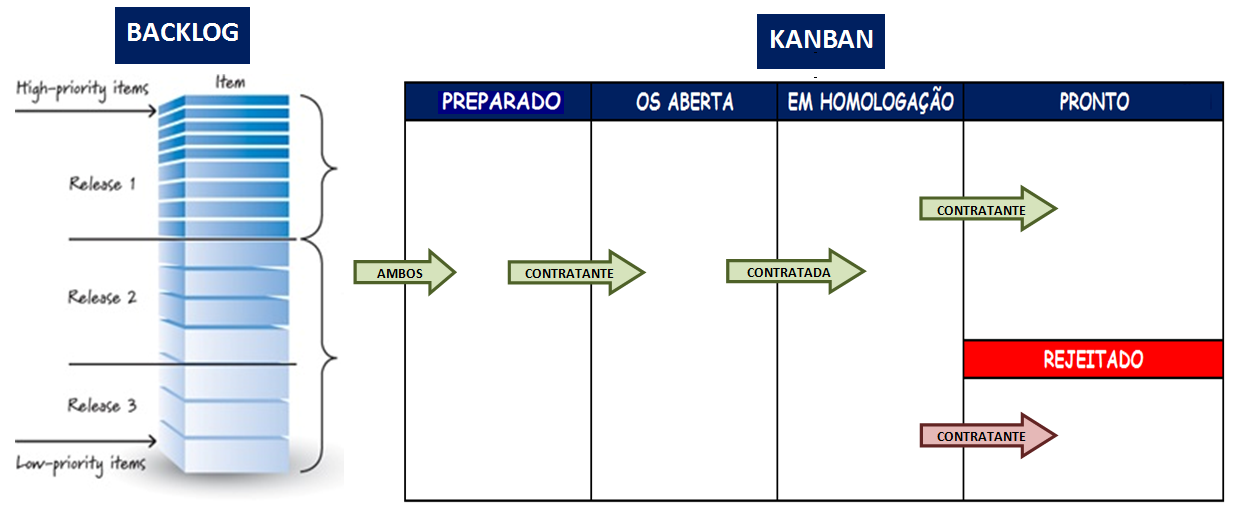
\includegraphics[scale=0.5]{figuras/kanbanIPHAN1.png}
		\caption{Quadro Kanban  \cite{parente}}
\end{figure}

A primeira raia do Kanban diz respeito aos itens que estão no estado “Preparado”. A condição de transição para esta raia pode ser feita da forma que o órgão quiser (Fig. 13). Por exemplo, os itens com mais prioridade podem ser os primeiros a irem para esta coluna. É importante que a definição de “Preparado” e a definição de “Pronto” estejam bem claras para todos os envolvidos.

\begin{figure}[H]
		\centering
		\label{fig06}
			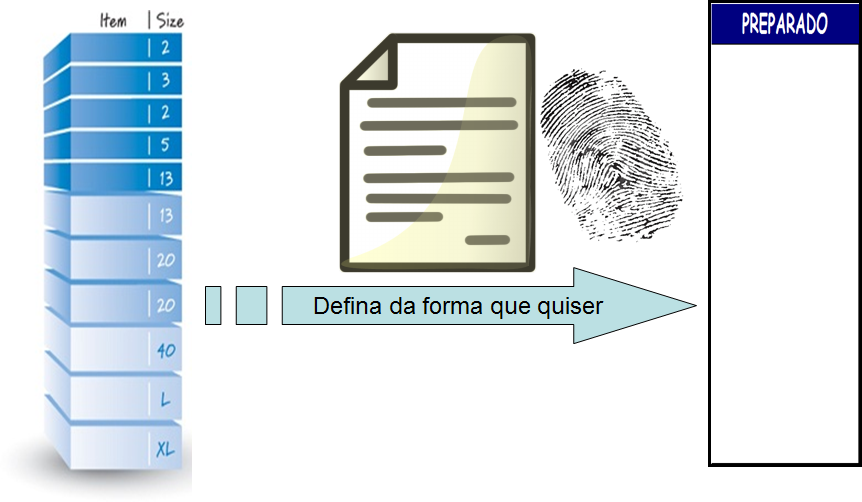
\includegraphics[scale=0.5]{figuras/kanbanIPHAN2.png}
		\caption{Transição para a raia Preparado \cite{parente}}
\end{figure}

A transição de um item da raia “Preparado” para a raia “OS Aberta” ocorre na abertura de uma ordem de serviço (Fig. 14). Ao observar o processo do MIDAS, percebe-se que essa transição ocorre após o planejamento da \textit{sprint}, no subprocesso \textit{Sprint}, onde uma ordem de serviço de desenvolvimento é aberta  com os itens que devem ser desenvolvidos para aquela \textit{sprint} e o desenvolvimento é iniciado. 

\begin{figure}[H]
		\centering
		\label{fig07}
			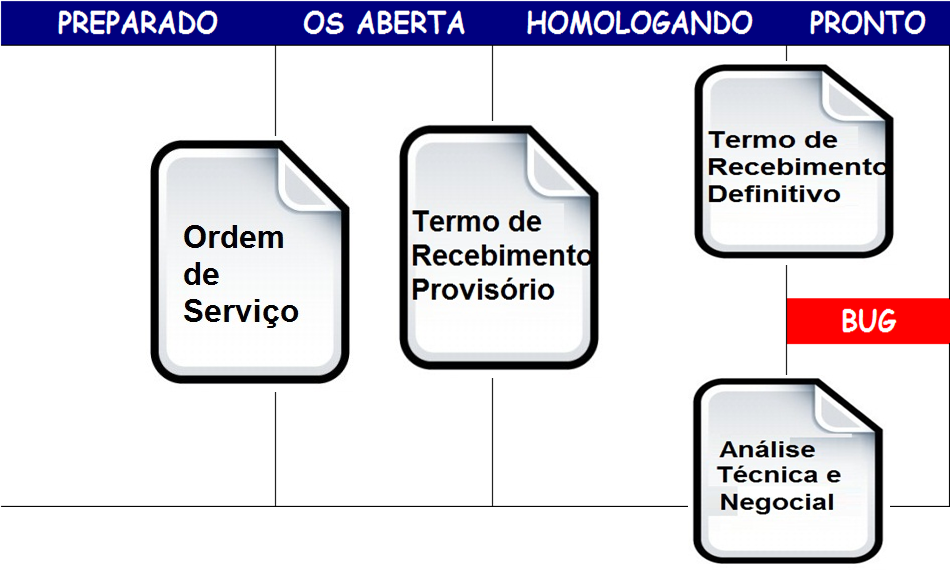
\includegraphics[scale=0.5]{figuras/kanbanIPHAN3.png}
		\caption{Transição entre raias \cite{parente}}
\end{figure}

A transição da raia “OS Aberta” para a raia “Homologando” ocorre quando o Termo de Recebimento Provisório é emitido (Fig. 14). Ao se observar o subprocesso de Realizar Ateste Técnico, percebe-se que essa transição ocorre na atividade “Receber Produtos”. Esta tem como entrada a ordem de serviço da fase e como saída o termo de recebimento provisório. Com a emissão do termo de recebimento provisório, os produtos recebidos entram na processo de homologação. 

A transição da raia “Homologando” para a raia “Pronto” ocorre quando o Termo de Recebimento Definitivo é emitido, ou seja, quando todos os produtos que foram anteriormente entregues são verificados e aprovados (Fig. 14). Para tanto são aferidos a aderência aos padrões técnicos e aos requisitos a partir de uma análise técnica e negocial, realizadas conjuntamente pelo Fiscal do Contrato e o Gestor de Negócio. Se forem detectados defeitos nos produtos entregues ou se eles forem rejeitados ou tiverem necessidade de refatoração, eles retornam para a fila de demandas, iniciando novamente o ciclo. A sinalização de rejeitado ou \textit{bug} diz respeito a funcionalidade que foi rejeitada por não atender o que foi pedido tanto funcionalmente quanto tecnicamente. A sinalização de refatoração diz respeito a mudança que é pedida em uma funcionalidade depois de ela já ter sido implementada. Para que uma funcionalidade entre nessa sinalização é preciso que o gestor de negócio assuma a responsabilidade pelos impactos que a mudança causará no custo, tempo e escopo.

Vale ressaltar que é importante que o trabalho em progresso (WIP) seja limitado conforme o que é conceituado no método Kanban. O IPHAN definiu um limite de 200 Pontos por Função por ciclo de trabalho (Fig. 15). 

\begin{figure}[h]
		\centering
		\label{fig08}
			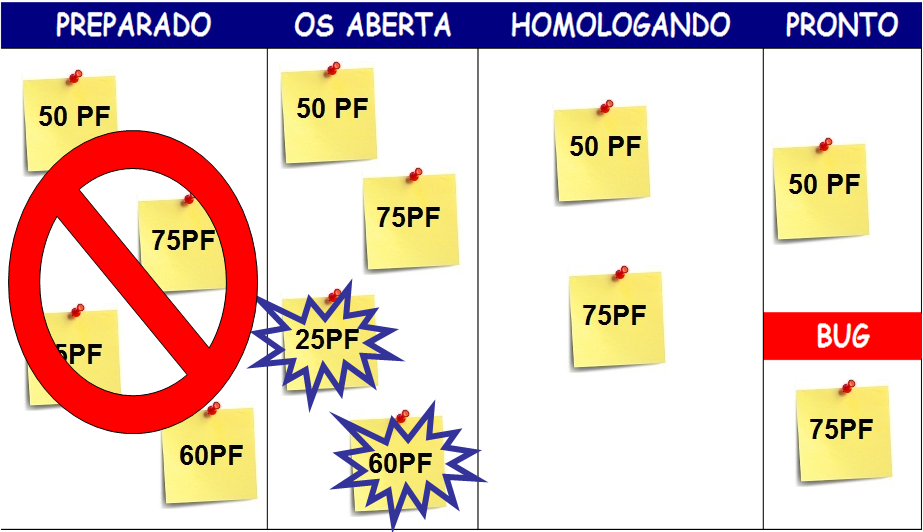
\includegraphics[scale=0.5]{figuras/kanbanIPHAN4.png}
		\caption{Limitação de WIP \cite{parente}}
\end{figure}

É importante sempre valorizar a entrega de produto funcional e não pagar por apenas documentação. Assim, o IPHAN dividia a forma de pagamento da contratada em percentuais, de acordo com a fase, valorizando a fase de execução, como ilustrado na Tab. (2).


\begin{table}[H]
\center
\footnotesize
\begin{tabular}{|p{6cm}|p{6cm}|}
  \hline
   \textbf{Fase} & \textbf{Percentual de Pagamento}\\
    \hline
   Planejamento (1 vez) & 5\%\\
   \hline    
   Execução (n vezes) & 80\%\\
    \hline
   Encerramento (1 vez) & 15\%\\
   \hline
\end{tabular}
\caption{Formas de Pagamento}
\end{table}


Outra técnica importante que foi construída diz respeito a parelização das atividades (Fig. 16). Enquanto uma ordem de serviço está na etapa de homologação, outra ordem de serviço pode ser preparada, evitando que o fluxo do processo pare e haja desperdício. 

\begin{figure}[H]
		\centering
		\label{fig09}
			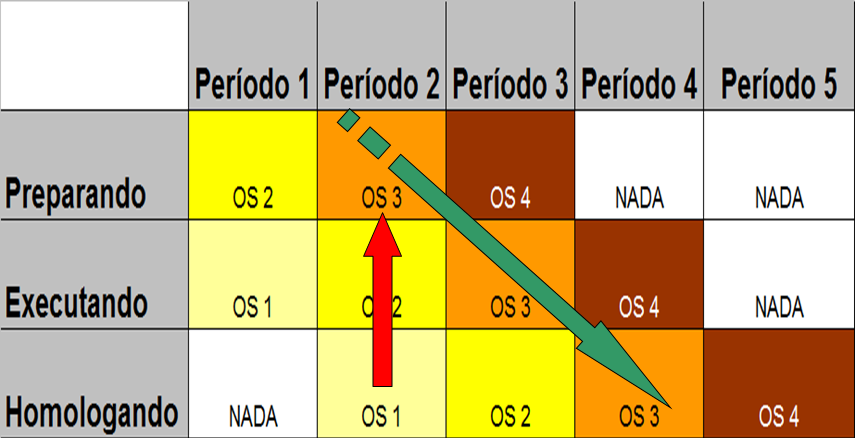
\includegraphics[scale=0.5]{figuras/kanbanIPHAN5.png}
		\caption{Parelização de Atividades \cite{parente}}
\end{figure}

O Kanban evidencia a aderência de utilização de métodos ágeis. A paralelização das atividades, que evita desperdícios de trabalho, evidencia a aderência ao Lean no Desenvolvimento de \textit{Software}. Assim, conclui-se que as premissas utilizadas como base para o desenvolvimento do Kanban foram baseadas tanto nos princípios ágeis quanto nos princípios do Lean. Após alguns meses de aplicação dessa solução o órgão deu início a construção da Metodologia IPHAN de Gestão de Demandas de Desenvolvimento Ágil de \textit{Software} (MIDAS). Uma parte do MIDAS pode ser visualizada no Anexo B. 



\section[Análise dos Dados]{Análise dos Dados}

\subsection[Efeitos sobre a entrega de ordens de serviço]{Efeitos sobre a entrega de ordens de serviço}

\subsection[Efeitos sobre a satisfação do cliente]{Efeitos sobre a satisfação do cliente}

O cliente do projeto SICG é representado pelo papel de dono do produto, que também atuou como gestor do contrato, e por todos os envolvidos no projeto por parte do IPHAN. Os IPHAN nunca havia participado anteriormente de um projeto onde a gestão do contrato era realizada com o uso de métodos ágeis, portanto, a experiência dos envolvidos no projeto com métodos ágeis era pouca. Para coletar a opinião do cliente acerca das questões de pesquisa QE10  e QE11 foi aplicado um questionário.

A Figura \ref{visibilidade} apresenta a visibilidade do processo de todos os envolvidos no projeto por parte do IPHAN. Cerca de 80\% dos envolvidos no projeto considerou a visibilidade do processo como "Alta", dentre eles o gestor do contrato.

\begin{figure}[H]
		\centering
			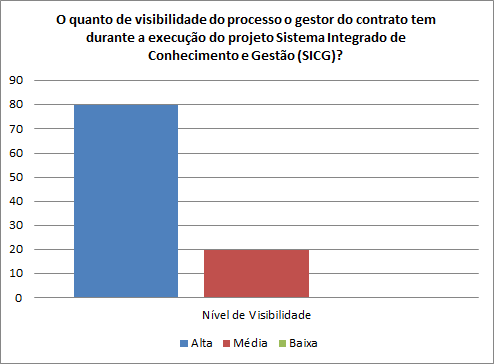
\includegraphics[scale=1.0]{figuras/visibilidade.png}
		\caption{Nível de Visibilidade do Processo do Projeto SICG}
		\label{visibilidade}
\end{figure}

A Figura \ref{satisfacao} apresenta o resultado de satisfação do IPHAN com relação ao produto entregue. De forma unânime foi considerado como "Satisfeito" o produto entregue pela empresa contratada. 

\begin{figure}[H]
		\centering
			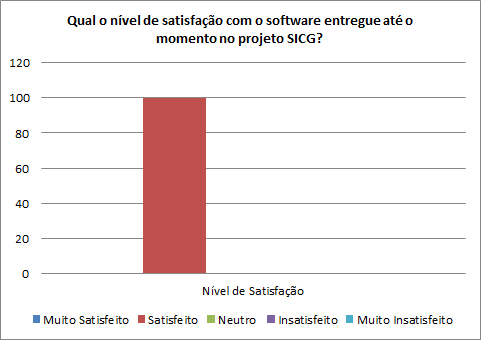
\includegraphics[scale=1.0]{figuras/satisfacao.png}
		\caption{Nível de Satisfação do Produto Entregue do Projeto SICG}
		\label{satisfacao}
\end{figure}

\subsection[Efeitos sobre a qualidade do código]{Efeitos sobre a qualidade do código}

A qualidade do código fonte do SICG pode ser avaliada por meio de métricas. Neste trabalho foram selecionadas as métricas de código fonte levantadas e categorizadas por MEIRELLES: métricas de tamanho e complexidade e métricas de orientação à objetos. 

As métricas de tamanho e complexidade selecionadas são: 

\textbf{LOC (Lines of Code):} número de Linhas de Código foi uma das primeiras métricas
utilizadas para medir o tamanho de um software. São contadas apenas as linhas
executáveis, ou seja, são excluídas linhas em branco e comentários (JONES,
1991).

 \vspace{\onelineskip} 

\textbf{ACCM (Average Cyclomatic Complexity per Method):} média da Complexidade
Ciclomática por Método mede a complexidade dos métodos ou funções
de um programa. Essa métrica pode ser representada através de um grafo de fluxo
de controle (MCCABE, 1976). O uso de estruturas de controle, tais como, if, else,
while aumentam a complexidade ciclomática de um método.

 \vspace{\onelineskip} 

As métricas de orientação à objetos selecionadas são:

\textbf{ACC (Afferent Connections per Class):} conexões Aferentes por Classe é o número
total de classes externas de um pacote que dependem de classes de dentro desse
pacote. Quando calculada no nível da classe, essa medida também é conhecida como
Fan-in da classe, medindo o número de classes das quais a classe é derivada e, assim,
valores elevados indicam uso excessivo de herança múltipla (MCCABE; DREYER;
WATSON, 1994) (CHIDAMBER; KEMERER, 1994).

 \vspace{\onelineskip} 

\textbf{RFC (Response For a Class):} respostas para uma Classe é número de métodos
dentre todos os métodos que podem ser invocados em resposta a uma mensagem
enviada por um objeto de uma classe (SHARBLE; COHEN, 1993).

 \vspace{\onelineskip} 

\textbf{LCOM4 (Lack of Cohesion in Methods):} falta de Coesão entre Métodos. Originalmente
proposto por Chidamber e Kemerer (1994) como LCOM não teve uma
grande aceitabilidade. Após críticas e sugestões a métrica foi revisada por Hitz e
Montazeri (1995), que propôs a LCOM4. Para calcular LCOM4 de um módulo, é
necessário construir um gráfico não-orientado em que os nós são os métodos e atributos
de uma classe. Para cada método, deve haver uma aresta entre ele e um outro
método ou variável que ele usa. O valor da LCOM4 é o número de componentes
fracamente conectados nesse gráfico.

 \vspace{\onelineskip} 

\textbf{NOM (Number of Methods):} número de Métodos é usado para medir o tamanho
das classes em termos das suas operações implementadas. Essa métrica é usada para
ajudar a identificar o potencial de reúso de uma classe. Em geral, as classes com
um grande número de métodos são mais difíceis de serem reutilizadas, pois elas são
propensas a serem menos coesas (LORENZ; KIDD, 1994).

 \vspace{\onelineskip} 

\textbf{DIT (Depth of Inheritance Tree):} profundidade da Árvore de Herança é o número
de superclasses ou classes ancestrais da classe sendo analisada. São contabilizadas
apenas as superclasses do sistema, ou seja, as classes de bibliotecas não são
contabilizadas. Nos casos onde herança múltipla é permitida, considera-se o maior
caminho da classe até uma das raízes da hierarquia. Quanto maior for o valor DIT,
maior é o número de atributos e métodos herdados, e, portanto,maior é a complexidade
(SHIH et al., 1997).

 \vspace{\onelineskip} 

\textbf{NOC (Number of Children):} número de Filhos é o número de subclasses ou classes
filhas que herdam da classe analisada (ROSENBERG; HYATT, 1997). Deve se ter
cautela ao modificar classes com muitos filhos, pois uma simples modificação de
assinatura de um método, pode criar uma mudança em muitas classes.

 \vspace{\onelineskip} 

Um dos objetivos científicos do estudo de Meirelles foi a identificação das distribuições estatísticas do valores das métricas apresentadas anteriormente em 38 projetos
de software livre. A partir de cada uma das distribuições estatísticas Meirelles classificou as métricas de código fonte de acordo com a frequência dos valores apresentados,
com os intervalos: muito frequente, frequente, pouco frequente e não frequente. Para simplificar o entendimento das métricas de código fonte, Morais interpretou os rótulos dos
intervalos de frequência definidos por Meirelles em em rótulos qualitativos, tal como a Tabela 4. 

\begin{table}[!ht]
	\begin{center}
	 \begin{tabular}{|l|l|}
		\hline
		Intervalo de Frequência & Intervalos Qualitativos \\ \hline
		Muito Frequente & Excelente \\ \hline
		Frequente       & Bom       \\ \hline
		Pouco Frequente & Regular   \\ \hline
		Não Frequente   & Ruim      \\ \hline
		\end{tabular}
		\caption{Nome dos Intervalos de Frequência e Qualitativos}
		\label{nomes}
		\end{center}
		\end{table}


Posteriormente, apresenta-se a Tabela 3, retirada do
estudo de Meirelles (2013), com os intervalos encontrados para C++ e Java. Com isso, os intervalos apresentados na Tabela 5 foram os utilizados como os indicadores
de qualidade de código fonte na análise deste estudo de caso. É importante ressaltar que quando apresentarmos o resultado da análise sobre o código fonte desse estudo de caso e dissermos que o código fonte tem um rótulo "excelente" ou "ruim" para determinada métrica siginifica que esse código fonte é "excelente" ou "ruim" em comparação ao melhor projeto de software livre selecionado por Meirelles na Linguagem Java, que foi o Eclipse.

\begin{table}[!ht]
	\begin{center}
	\begin{tabular}{ |l|l|l|l| }
		\hline
		Métrica & Intervalo Qualitativo & Java & C++ \\ \hline
		%-------------------------------
		\multirow{4}{*}{LOC} 
		 & Excelente & [de 0 a 33] & [de 0 a 31] \\
		 & Bom & [de 34 a 87] & [de 32 a 84] \\
		 & Regular & [de 88 a 200] & [de 85 a 207] \\
		 & Ruim & [acima de 200] & [acima de 207] \\ \hline
		 %---------------------------------

		 %-------------------------------
		\multirow{4}{*}{ACCM} 
		 & Excelente & [de 0 a 2,8] & [de 0 a 2,0] \\
		 & Bom & [de 2,9 a 4,4] & [de 2,1 a 4,0] \\
		 & Regular & [de 4,5 a 6,0] & [de 4,1 a 6,0] \\
		 & Ruim & [acima de 6] & [acima de 6] \\ \hline
		 %---------------------------------


		%-------------------------------
		\multirow{4}{*}{ACC} 
		 & Excelente & [de 0 a 1] & [de 0 a 2,0] \\
		 & Bom & [de 1,1 a 5] & [de 2,1 a 7,0] \\
		 & Regular & [de 5,1 a 12] & [de 7,1 a 15] \\
		 & Ruim & [acima de 12] & [acima de 15] \\ \hline
		 %---------------------------------


		%-------------------------------
		\multirow{4}{*}{RFC} 
		 & Excelente & [de 0 a 9] & [de 0 a 29] \\
		 & Bom & [de 10 a 26] & [de 30 a 64] \\
		 & Regular & [de 27 a 59] & [de 65 a 102] \\
		 & Ruim & [acima de 59] & [acima de 102] \\ \hline
		 %---------------------------------

		 %-------------------------------
		\multirow{4}{*}{LCOM4} 
		 & Excelente & [de 0 a 3] & [de 0 a 5] \\
		 & Bom & [de 4 a 7] & [de 6 a 10] \\
		 & Regular & [de 8 a 12] & [de 11 a 14] \\
		 & Ruim & [acima de 12] & [acima de 14] \\ \hline
		 %---------------------------------

		 %-------------------------------
		\multirow{4}{*}{NOM} 
		 & Excelente & [de 0 a 8] & [de 0 a 10] \\
		 & Bom & [de 9 a 17] & [de 11 a 17] \\
		 & Regular & [de 18 a 27] & [de 18 a 26] \\
		 & Ruim & [acima de 27] & [acima de 26] \\ \hline
		 %---------------------------------

		 %-------------------------------
		\multirow{4}{*}{DIT} 
		 & Excelente & [de 0 a 2] & [de 0 a 1] \\
		 & Bom & [de 3 a 4] & [de 2 a 3] \\
		 & Regular & [de 5 a 6] & [de 3 a 4] \\
		 &
		  Ruim & [acima de 6] & [acima de 4] \\ \hline
		 %---------------------------------

		%-------------------------------
		\multirow{4}{*}{NOC} 
		 & Excelente & [de 0 a 1] & [0] \\
		 & Bom & [de 1 a 2] & [1] \\
		 & Regular & [de 2 a 3] & [de 1 a 2] \\
		 & Ruim & [acima de 3] & [acima de 2] \\ \hline
		 %---------------------------------

	\end{tabular}
	\caption{Intervalos das Métricas para Java e C++}
	\label{metrics}
	\end{center}
	\end{table}

De forma geral, o processo realizado para a análise do código fonte do SICG foi retirado do trabalho desenvolvido por BAUFAKER, que  consiste em: executar a ferramenta Analizo sobre o código fonte do projeto SICG, o qual resultará em um arquivo .csv com os resultados númericos das métricas selecionadas, transformar o arquivo .csv em json e inserir esse arquivo na arquitetura desenvolvida por BAUFAKER na ferramenta Pentaho. Ao final desse processo, temos como resultado os gráficos para análise. 

A fim de responder a questão de pesquisa QE12 serão mostrados a seguir os resultados do processamento do código fonte do projeto SICG no que diz respeito a qualidade do código ao longo das sprints do projeto de acordo com as oito métricas selecionadas. Os rótulos de intervalos de qualidade mostrados são resultantes dos valores médios de cada métrica para todas as classes do projeto. 

A Figura \ref{metricasprint} mostra os valores de todas as métricas ao longo das sprints do projeto. A seguir, serão apresentados os gráficos, primeiramente, dos resultados de cada métrica de forma individual ao longo das sprints do projeto e, posteriormente, o resultado geral da qualidade do código ao longo das sprints do projeto.

\begin{figure}[H]
		\centering
			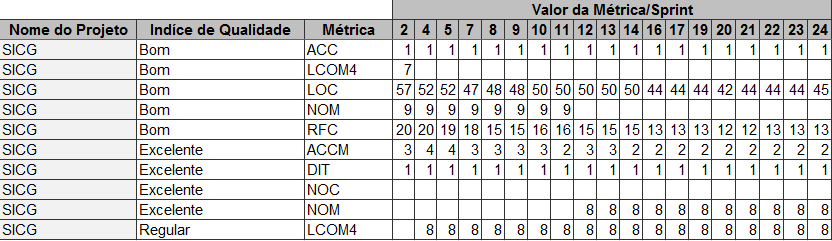
\includegraphics[scale=0.8]{figuras/metricasprint.png}
		\caption{Valores das Métricas do Projeto SICG}
		\label{metricasprint}
\end{figure}


\textbf{LOC (Lines of Code)}

A Figura \ref{loc} mostra a qualidade da métrica LOC. Esta métrica permanece com o intervalo de qualidade "Bom" constante ao longo das sprints do projeto.

\begin{figure}[H]
		\centering
			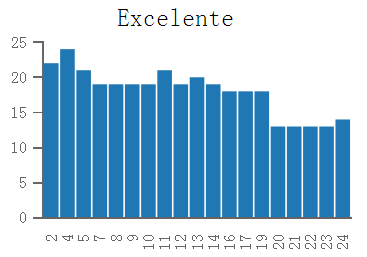
\includegraphics[scale=0.4]{figuras/loc.png}
		\caption{Qualidade da Métrica LOC nas Sprints do Projeto SICG}
		\label{loc}
\end{figure}

\textbf{ACCM (Average Cyclomatic Complexity per Method)}

A Figura \ref{accm} mostra a qualidade da métrica ACCM. Esta métrica permanece com o intervalo de qualidade "Excelente" constante ao longo das sprints do projeto.

\begin{figure}[H]
		\centering
			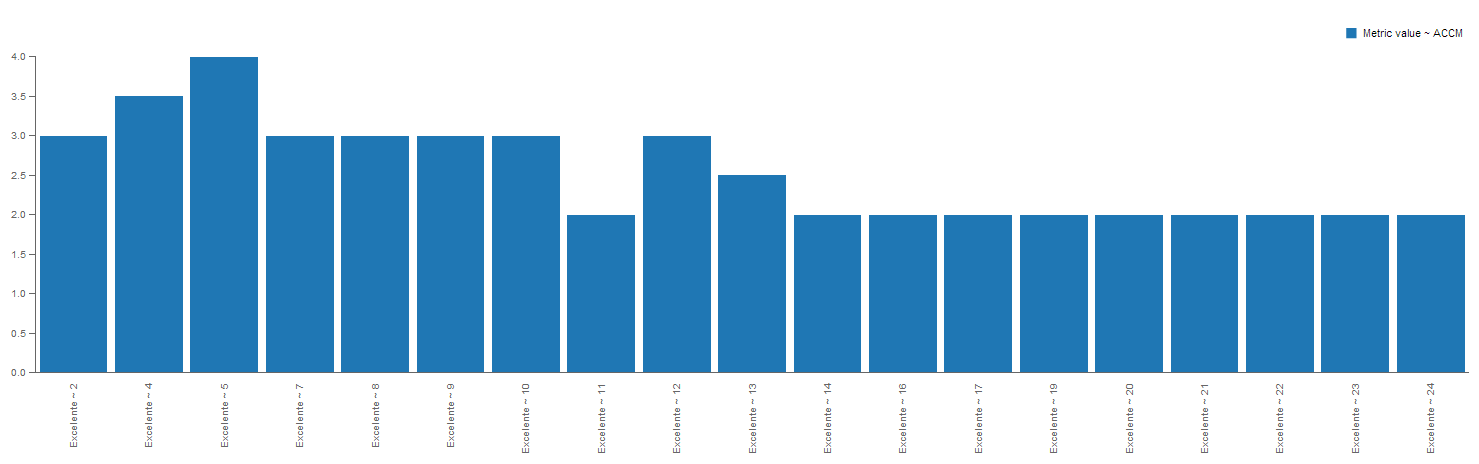
\includegraphics[scale=0.4]{figuras/accm.png}
		\caption{Qualidade da Métrica ACCM nas Sprints do Projeto SICG}
		\label{accm}
\end{figure}

\textbf{ACC (Afferent Connections per Class)}

A Figura \ref{acc} mostra a qualidade da métrica ACC. Esta métrica permanece com o intervalo de qualidade "Bom" constante ao longo das sprints do projeto.

\begin{figure}[H]
		\centering
			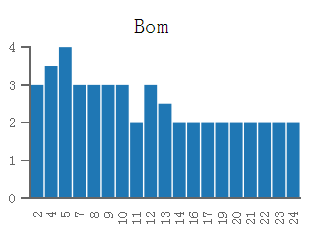
\includegraphics[scale=0.4]{figuras/acc.png}
		\caption{Qualidade da Métrica ACC nas Sprints do Projeto SICG}
		\label{acc}
\end{figure}

\textbf{RFC (Response For a Class)} 

A Figura \ref{rfc} mostra a qualidade da métrica RFC. Esta métrica permanece com o intervalo de qualidade "Bom" constante ao longo das sprints do projeto.

\begin{figure}[H]
		\centering
			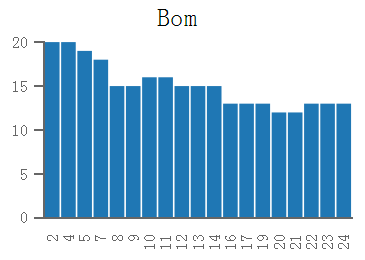
\includegraphics[scale=0.4]{figuras/rfc.png}
		\caption{Qualidade da Métrica RFC nas Sprints do Projeto SICG}
		\label{rfc}
\end{figure}

\textbf{LCOM4 (Lack of Cohesion in Methods)} 

A Figura \ref{lcom4} mostra a qualidade da métrica LCOM4. Esta métrica inicia com o intervalo de qualidade "Bom" na primeira sprint e, posteriormente, permanece com o intervalo de qualidade "Regular" constante ao longo das demais sprints do projeto.

\begin{figure}[H]
		\centering
			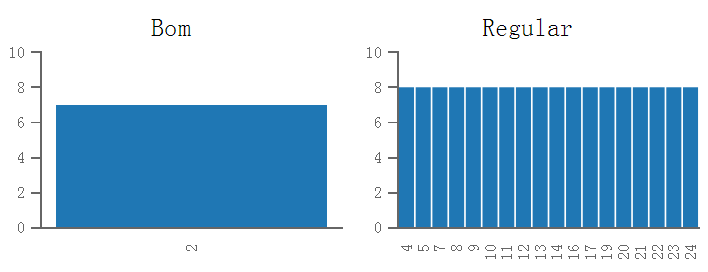
\includegraphics[scale=0.4]{figuras/lcom4.png}
		\caption{Qualidade da Métrica LCOM4  nas Sprints do Projeto SICG}
		\label{lcom4}
\end{figure}

\textbf{NOM (Number of Methods)} 

A Figura \ref{nom} mostra a qualidade da métrica NOM. Esta métrica permanece com o intervalo de qualidade "Bom" até a Sprint 11 do projeto, a partir da Sprint 12 o código fonte obtém uma melhoria e a métrica NOM passa a ter o intervalo de qualidade "Excelente" até a última sprint analisada do projeto.

\begin{figure}[H]
		\centering
			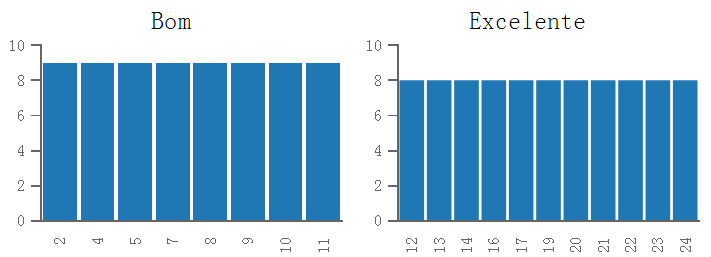
\includegraphics[scale=0.4]{figuras/nom.png}
		\caption{Qualidade da Métrica NOM nas Sprints do Projeto SICG}
		\label{nom}
\end{figure}

\textbf{DIT (Depth of Inheritance Tree)}

A Figura \ref{dit} mostra a qualidade da métrica DIT. Esta métrica permanece com o intervalo de qualidade "Excelente" constante ao longo das sprints do projeto.

\begin{figure}[H]
		\centering
			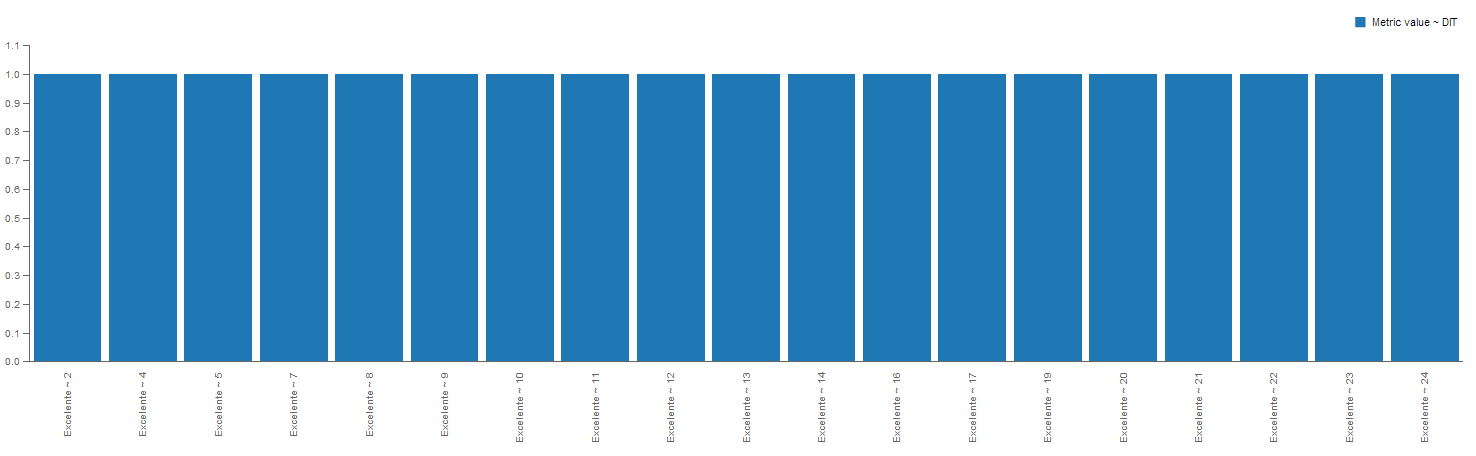
\includegraphics[scale=0.4]{figuras/dit.png}
		\caption{Qualidade da Métrica DIT nas Sprints do Projeto SICG}
		\label{dit}
\end{figure}

\textbf{NOC (Number of Children)}

A Figura \ref{noc} mostra a qualidade da métrica NOC. Esta métrica permanece com o intervalo de qualidade "Excelente" constante ao longo das sprints do projeto.

\begin{figure}[H]
		\centering
			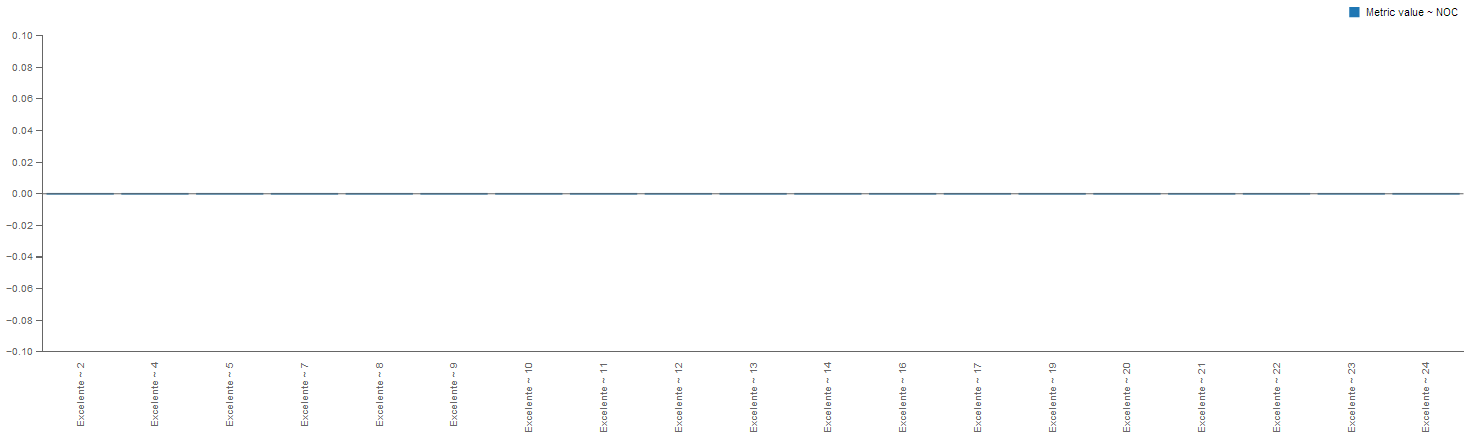
\includegraphics[scale=0.4]{figuras/noc.png}
		\caption{Qualidade da Métrica NOC nas Sprints do Projeto SICG}
		\label{noc}
\end{figure}

A Figura \ref{qualidadesprint} mostra a qualidade de todas as métricas analisadas ao longo das sprints do projeto. Considerando que a Sprint 24 é a última sprint do projeto e, portanto, seria o código final, observamos uma predominância do intervalo de qualidade "Excelente", seguido do intervalo "Bom" e "Regular", respectivamente. 

\begin{figure}[H]
		\centering
			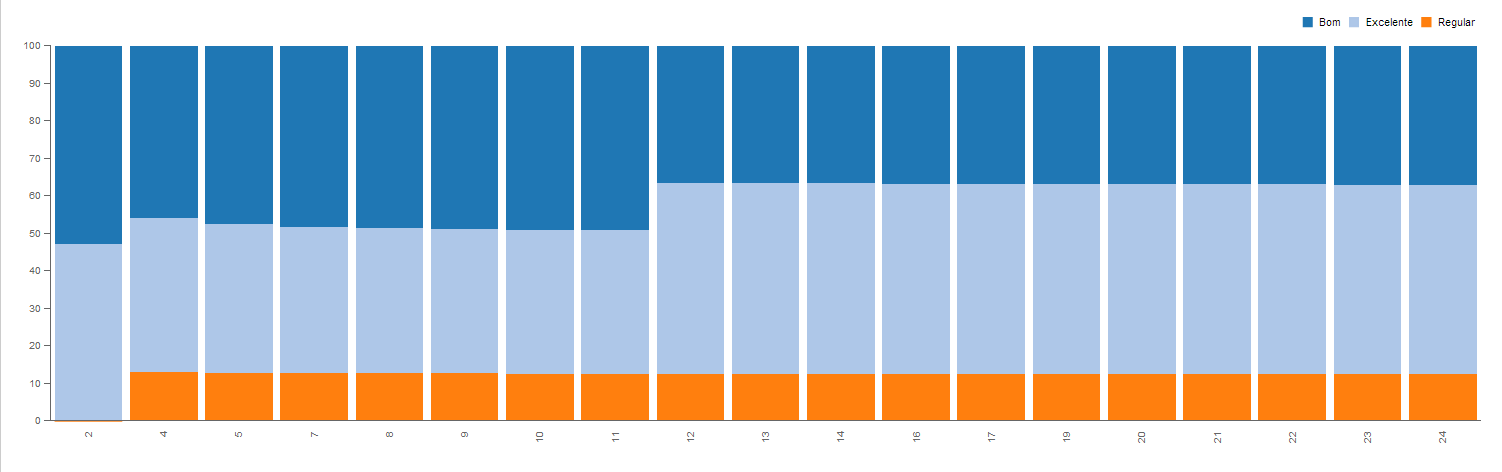
\includegraphics[scale=0.4]{figuras/qualidadesprint.png}
		\caption{Qualidade Geral das Métricas do Projeto SICG}
		\label{qualidadesprint}
\end{figure}


A Figura \ref{percepcaoqualidade} mostra a percepção da qualidade do código fonte do SICG segundo os envolvidos no projeto (Scrum Master, Product Owner, Gestor do Contrato, Coordenador do Projeto, Fiscal Técnico e Desenvolvedores). Cerca de 66\% dos envolvidos consideraram  o intervalo de qualidade do código como "Excelente" e os demais consideraram
o intervalo de qualidade como "Bom".

\begin{figure}[H]
		\centering
			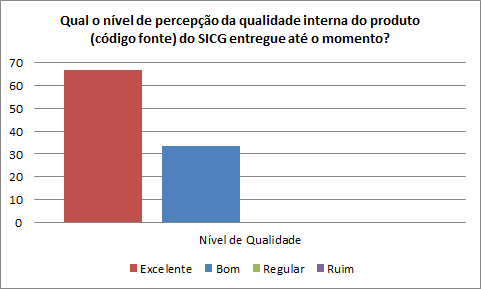
\includegraphics[scale=1.0]{figuras/percepcaoqualidade.png}
		\caption{Nível de Percepção da Qualidade do Código Fonte}
		\label{percepcaoqualidade}
\end{figure}

Assim, no que diz respeito a análise estática do código realizada, a qualidade do código fonte do projeto é satisfatória ao compararmos com o melhor software livre encontrado na linguagem de programação Java, o Eclipse, e também é satisfatória na percepção dos envolvidos no projeto SICG. 

\section[Resultados]{Resultados}

